%\documentclass[10pt, twocolumn]{article}
\documentclass[twocolumn,showpacs,preprintnumbers,amsmath,amssymb,prd]{revtex4}
%\documentclass[11 pt,preprint,preprintnumbers,amsmath,amssymb, prd]{revtex4}

% Preamble adapted from Surjeet Rajendran

\usepackage{latexsym}
\usepackage{amssymb}
\usepackage{epsfig,amsmath,graphics}
\usepackage{epstopdf}
\usepackage{verbatim}
\usepackage{wasysym}
\usepackage{hyperref}
\usepackage{feynmp-auto} % feynman diagrams
%\usepackage{subfig}
\usepackage[utf8]{inputenc}
\usepackage{xpatch}
\usepackage{xcolor}
\hypersetup{
    colorlinks,
    linkcolor={red!80!black},
    citecolor={green!60!black},
    urlcolor={blue!60!black}
}
\usepackage{appendix}

\newcommand{\OO}{\mathcal{O}}
\newcommand{\LL}{\mathcal{L}}
\newcommand{\HH}{\mathcal{H}}

\newcommand{\GeV}{\text{GeV}}
\newcommand{\MeV}{\text{MeV}}
\newcommand{\keV}{\text{keV}}
\newcommand{\rad}{\text{rad}}
\newcommand{\cm}{\text{cm}}
\newcommand{\angstrom}{\buildrel _{\circ} \over {\mathrm{A}}}
\newcommand{\pslash}{p\hspace{-0.070in}/\,}
\newcommand{\Mpl}{M_{\text{pl}}}
\newcommand{\ket}[1]{\ensuremath{\left|#1\right>}}
\newcommand{\bra}[1]{\ensuremath{\left<#1\right|}}
\newcommand{\braket}[2]{\ensuremath{\left<#1|#2\right>}}
%Large Parentheses
\def\r{\right)}
\def\l{\left(}

\begin{document}

\title{White Dwarfs as Dark Matter Detectors}


\author{Ryan Janish}
\affiliation{Berkeley Center for Theoretical Physics, Department of Physics,
University of California, Berkeley, CA 94720, USA}

\author{Vijay Narayan}
\affiliation{Berkeley Center for Theoretical Physics, Department of Physics,
University of California, Berkeley, CA 94720, USA}

\author{Paul Riggins}
\affiliation{Berkeley Center for Theoretical Physics, Department of Physics,
University of California, Berkeley, CA 94720, USA}

\begin{abstract}

White dwarfs can serve as detectors for ultra-heavy dark matter states which interact to trigger type Ia supernovae. This was originally proposed in \cite{Graham:2015apa} and used to  place bounds on primordial black holes. In this paper we extend the capability of white dwarf detectors to candidates with non-gravitational couplings, focusing on dark matter transits and collisions within the white dwarf. In particular, we provide a detailed analysis of the explosiveness for any heating mechanism in the white dwarf which releases high-energy standard model particles. We apply this mechanism to constrain Q-ball dark matter \textcolor{blue}{and model of dark nuclei} in regions of parameter space fundamentally inaccessible to terrestrial-based experiments.

\end{abstract}
\maketitle


\section{Introduction}
\label{sec:Introduction}

The detection of ultra-heavy dark matter (DM) is an open problem which will ultimately require a confluence of astrophysical probes. For instance, DM masses above $\sim 10^{22} ~\GeV$ will register fewer than 1 event per year in a typical terrestrial detector of size $\sim (100 ~\text{m})^2$. Furthermore, the lack of conclusive signatures on a variety of experimental fronts has led many to seriously consider DM candidates far above the weak scale and their potential signatures \textcolor{blue}{cite people}. One possibility proposed by \cite{Graham:2015apa} is that ultra-heavy DM can trigger supernovae in sub-Chandrasekhar white dwarf (WD) stars by inducing runaway fusion.  In this regard, white dwarfs can serve as detectors for ultra-heavy DM states.

White dwarfs are particularly suited to this task, as they are more susceptible to runaway fusion than are main-sequence stars. Runaway fusion requires that two criteria be met: a region within the star must be hot enough to support exothermic fusion reactions, and the rate at which energy is released by these reactions must dominate any cooling mechanisms that drain energy from the fusing region.  The stellar medium of a WD has fewer cooling mechanisms available than does a non-degenerate star - WD cooling relies on thermal diffusion whereas main-sequence stars can also cool by thermal expansion.  This is suppressed in a WD since its pressure is determined by electron degeneracy and is thus independent of temperature. The remaining primary cooling mechanism, diffusion, becomes less important over longer length scales and can be overcome by sufficiently heating a large enough region of the WD.

The necessary trigger for runaway fusion was initially computed in \cite{Woosley} and recently implemented in \cite{Graham:2015apa} to constrain primordial black holes, which can ignite WD stars via gravitational dynamical friction.  In addition, the authors of \cite{Graham:2015apa} identify several other heating mechanisms involving DM which may be constrained in a similar manner. \textcolor{blue}{Some of these (compact cores) have been explored in...cite.}  In this work, we extend their analysis to DM candidates with non-gravitational couplings, focusing on DM transits through the WD and DM-DM collisions within the WD which release energy in the form of standard model (SM) particles. More generally, we provide a detailed analysis of the explosive power and resulting constraints on any DM with interactions of this sort.

Concrete examples of DM candidates with interactions of this type include baryonic Q-balls found in supersymmetric extensions of the SM and \textcolor{blue}{dark nuclei with high-order couplings to the SM.} We are able to constrain these models in regions of parameter space fundamentally inaccessible to terrestrial experiments. However, it is important to note that any such DM constraints are by nature complimentary to terrestrial ones - it is more massive DM that is likely to trigger supernovae, and also more massive DM that have sufficiently low flux on Earth. What allows the WD to be effective in this regime is its enhanced surface area $\sim (4000 ~\text{km})^2$ and exceptionally long lifetime $\sim \text{Gyr}$.
\textcolor{blue}{Other ignition sources exist (i.e., detector backgrounds). Discuss the specific tests we apply (WD lifetime, SN rate) to derive our constraints.}

We begin in Section~\ref{sec:Review} by reviewing the explosion mechanism in a WD. In Section~\ref{sec:DMexplode}, we parametrize the properties of DM necessary to trigger explosions through non-gravitational interactions in the case of a DM transit or collision in the star. The precise explosive power will be determined by a heating length, which is computed in Section~\ref{sec:HeatingLength} for different possible interactions. Following this general discussion, we apply the WD detector to place constraints on ultra-heavy dark matter in Section~\ref{sec:Constraints}, and apply these constraints in Section~\ref{sec:ConcreteExamples} to Q-balls as a concrete example. We conclude in Section~\ref{sec:discussion}.

\section{Runaway Fusion in a White Dwarf}
\label{sec:Review}

Nuclear fusion in a WD is controlled by two parameters, a \emph{fusion temperature} $T_f$ and a \emph{trigger size} $\lambda_T$.  The fusion temperature is set by the energy required for ions to overcome their mutual Coulomb barrier.  In carbon-oxygen WDs, this is a constant $T_f \sim \MeV$.  The trigger size is a measure of the effectiveness of WD cooling to quench fusion, which depending on stellar density is set by the thermal diffusivity of photons or degenerate electrons \cite{Woosley}.  The diffusive cooling timescale of a region increases with its linear size, whereas the fusion heating timescale is independent of size.  Thus there is a critical length scale, the trigger size $\lambda_T$, below which diffusive cooling controls the thermal evolution of a temperature peak and above which heat liberated by fusion dominates. Therefore, a heated region with temperature $T$ greater than $T_f$ and size $R$ greater than $\lambda_T$ in a sub-Chandrasekhar WD will launch a runaway fusion chain-reaction and result in a \textcolor{blue}{type Ia} supernova (SN):
\begin{equation}
\label{eq:runaway}
  T \gtrsim T_f, ~~~~ R \gtrsim \lambda_T.
\end{equation}
\textcolor{red}{check the common usage of ``type Ia"}  The value of $\lambda_T$ is highly sensitive to the WD density, and has been calculated numerically in \cite{Woosley} and analytically scaled for varying WD masses in \cite{Graham:2015apa}. As in \cite{Graham:2015apa}, we restrict our attention to carbon-oxygen WDs in the upper mass range $0.7 - 1.4 ~M_{\odot}$ which correspond to a number density of nuclei $n_\text{ion} \sim 10^{29} - 10^{32} ~\cm^{-3}$. Over this range, the trigger size is approximately $\lambda_T \sim 10^{-5} - 10^{-2} ~\text{cm}$.

A general energy deposition event in the WD can be described by an energy deposit $\mathcal{E}_0$ and heating length $L_0$.  After an appropriate thermalization time, this energy deposit will result in a local peak in the temperature profile - we take $\mathcal{E}_0$ to be the excess thermal energy within this initial peak and $L_0$ to be its characteristic length scale.  $L_0$ is determined by the efficiency with which the energy deposition mechanism interacts with the WD medium, and may vary significantly with deposition mechanism and WD density.  For example, suppose that kinetic energy was transferred directly to ions via short-range elastic scatters. These ions would thermalize over their collisional time scale, resulting in a heating length of order the ion mean free path. In the other extreme, suppose that a process produces electrons with energy just above the Fermi energy.  These electrons have Pauli-suppressed interactions with the medium and will travel a long distance before their energy is scattered and thermalized, resulting in a much larger $L_0$.

A given temperature peak will eventually ignite runaway fusion if at any time in its future thermal evolution it satisfies condition \eqref{eq:runaway}.  This will be true for a heating event if it initially deposits both sufficient total energy \emph{and} energy density.  We find the explosion condition for a heating event initially described by $\mathcal{E}_0$, $L_0$ to be:
\begin{equation}
\label{eq:boom}
  \mathcal{E}_0 \gtrsim n_\text{ion} T_f \text{max}\{L_0, \lambda_T\}^3
\end{equation}
where $n_\text{ion}$ is the number density of carbon ions in the WD. Note that there is an absolute minimum energy required to ignite a WD:
\begin{equation}
\label{eq:Eboom}
\mathcal{E}_{\text{boom}} \sim n_\text{ion} T_f \lambda_T^3 \sim 10^{14} - 10^{21} ~\GeV,
\end{equation}
where the trigger size $\lambda_T$ varies over a range of WD densities.  This is plotted in Figure \ref{fig:Eboom} as a function of WD mass \cite{website}.  The threshold \eqref{eq:Eboom} is only sufficient if the deposited energy thermalizes within a region of size $\lambda_T$.  If energy is deposited on a length scale larger than $\lambda_T$, the threshold for explosion may be parametrically larger.  As a result, understanding the heating length $L_0$ of a processes is critical to assessing whether or not it results in a SN.  This is the focus of Section~\ref{sec:HeatingLength}.

\begin{figure}
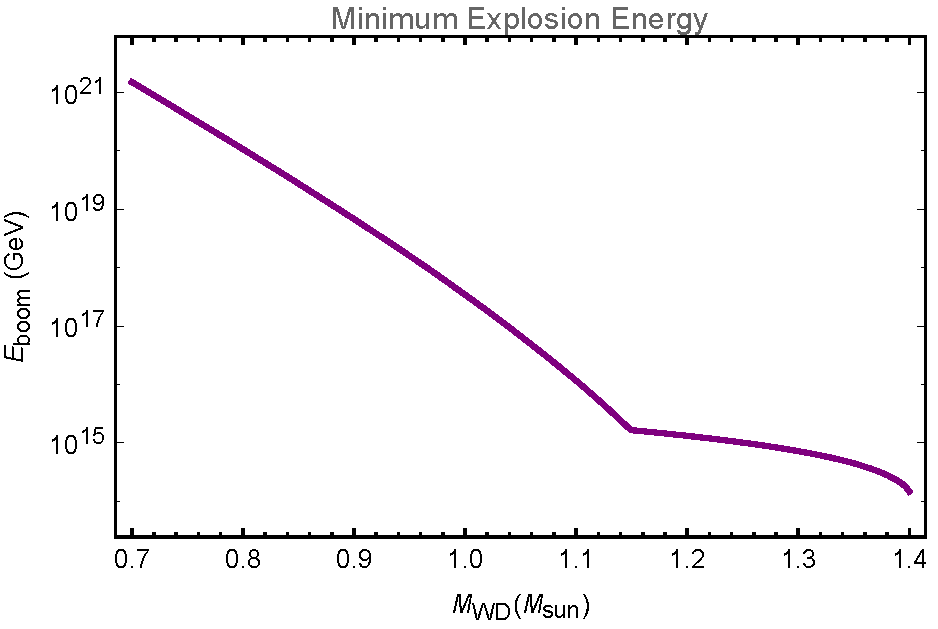
\includegraphics[scale=.45]{Eboom.pdf}
\caption{Minimum energy required to trigger explosion in a WD, based on numerical results for $\lambda_T$ \cite{Woosley}.}
\label{fig:Eboom}
\end{figure}

\section{Dark Matter Induced Ignition}
\label{sec:DMexplode}

In this section we discuss and parameterize the ability of non-gravitational dark matter interactions to trigger a supernova, focusing on interactions that cause heating through the production of high-energy SM particles in the WD. In particular, we seek a condition on the parameters of such interactions that determines whether or not a WD-DM encounter results in a SN.  Of course, finding such a condition requires knowledge of DM model-dependent subtleties, such as the nature of the SM states produced in the WD and the response of the DM to this interaction.  In what follows, we will outline this calculation in the general case and identify the necessary SM physics.  We then specialize to three physically expected and illustrative classes of DM-WD encounter: DM-DM collisions and DM decays within the star, and ``bullet-like" DM transits of a WD.  We will parameterize these encounters and derive their explicit explosion conditions. 

\subsection{General DM-WD Encounters}
We consider the encounter of a WD with a DM particle that possesses interactions as in Figure \ref{fig:feynman}.  These interactions result in some initial distribution in space and energy of SM particles, which must be computed from the details of the model, taking into account the trajectory of the DM particle through the star.  The produced SM particles will then travel some distance, giving up their energy to the stellar medium in a manner analogous to collider products in a calorimeter.  This is the deposition energy, resulting in local heating events as described in Section \ref{sec:Review}.  Depending of the details of the initial SM distribution, this may give rise to one temperature peak involving the energy of many produced particles, or a number of smaller, separated peaks.  In any case, the energy $\mathcal{E}_0$ of these deposits will be of order the initial kinetic energy of the SM particles involved.  The length $L_0$ of the deposit is set by the distance SM products travel before losing their kinetic energy to the medium (i.e., the \emph{range}), and the subsequent thermalization timescale of that energy within the medium.  This will depend on the SM species and its energy, as well as the stellar density.  With $\mathcal{E}_0$ and $L_0$ in hand, explosion is determined by condition \eqref{eq:boom}.  

The heating lengths of SM particles in the WD is a critical building-block for constraining any DM model in this fashion, and it involves purely SM physics.  To facilitate these constraints, we have calculated $L_0$ as a function of energy and stellar density for a representative set of SM species, presented in Section \ref{sec:HeatingLength}.  These calculations also reveal the types of DM-SM interactions most susceptible to inducing SN, which is further discussed below \textcolor{blue}{section reference?}.

\begin{figure}
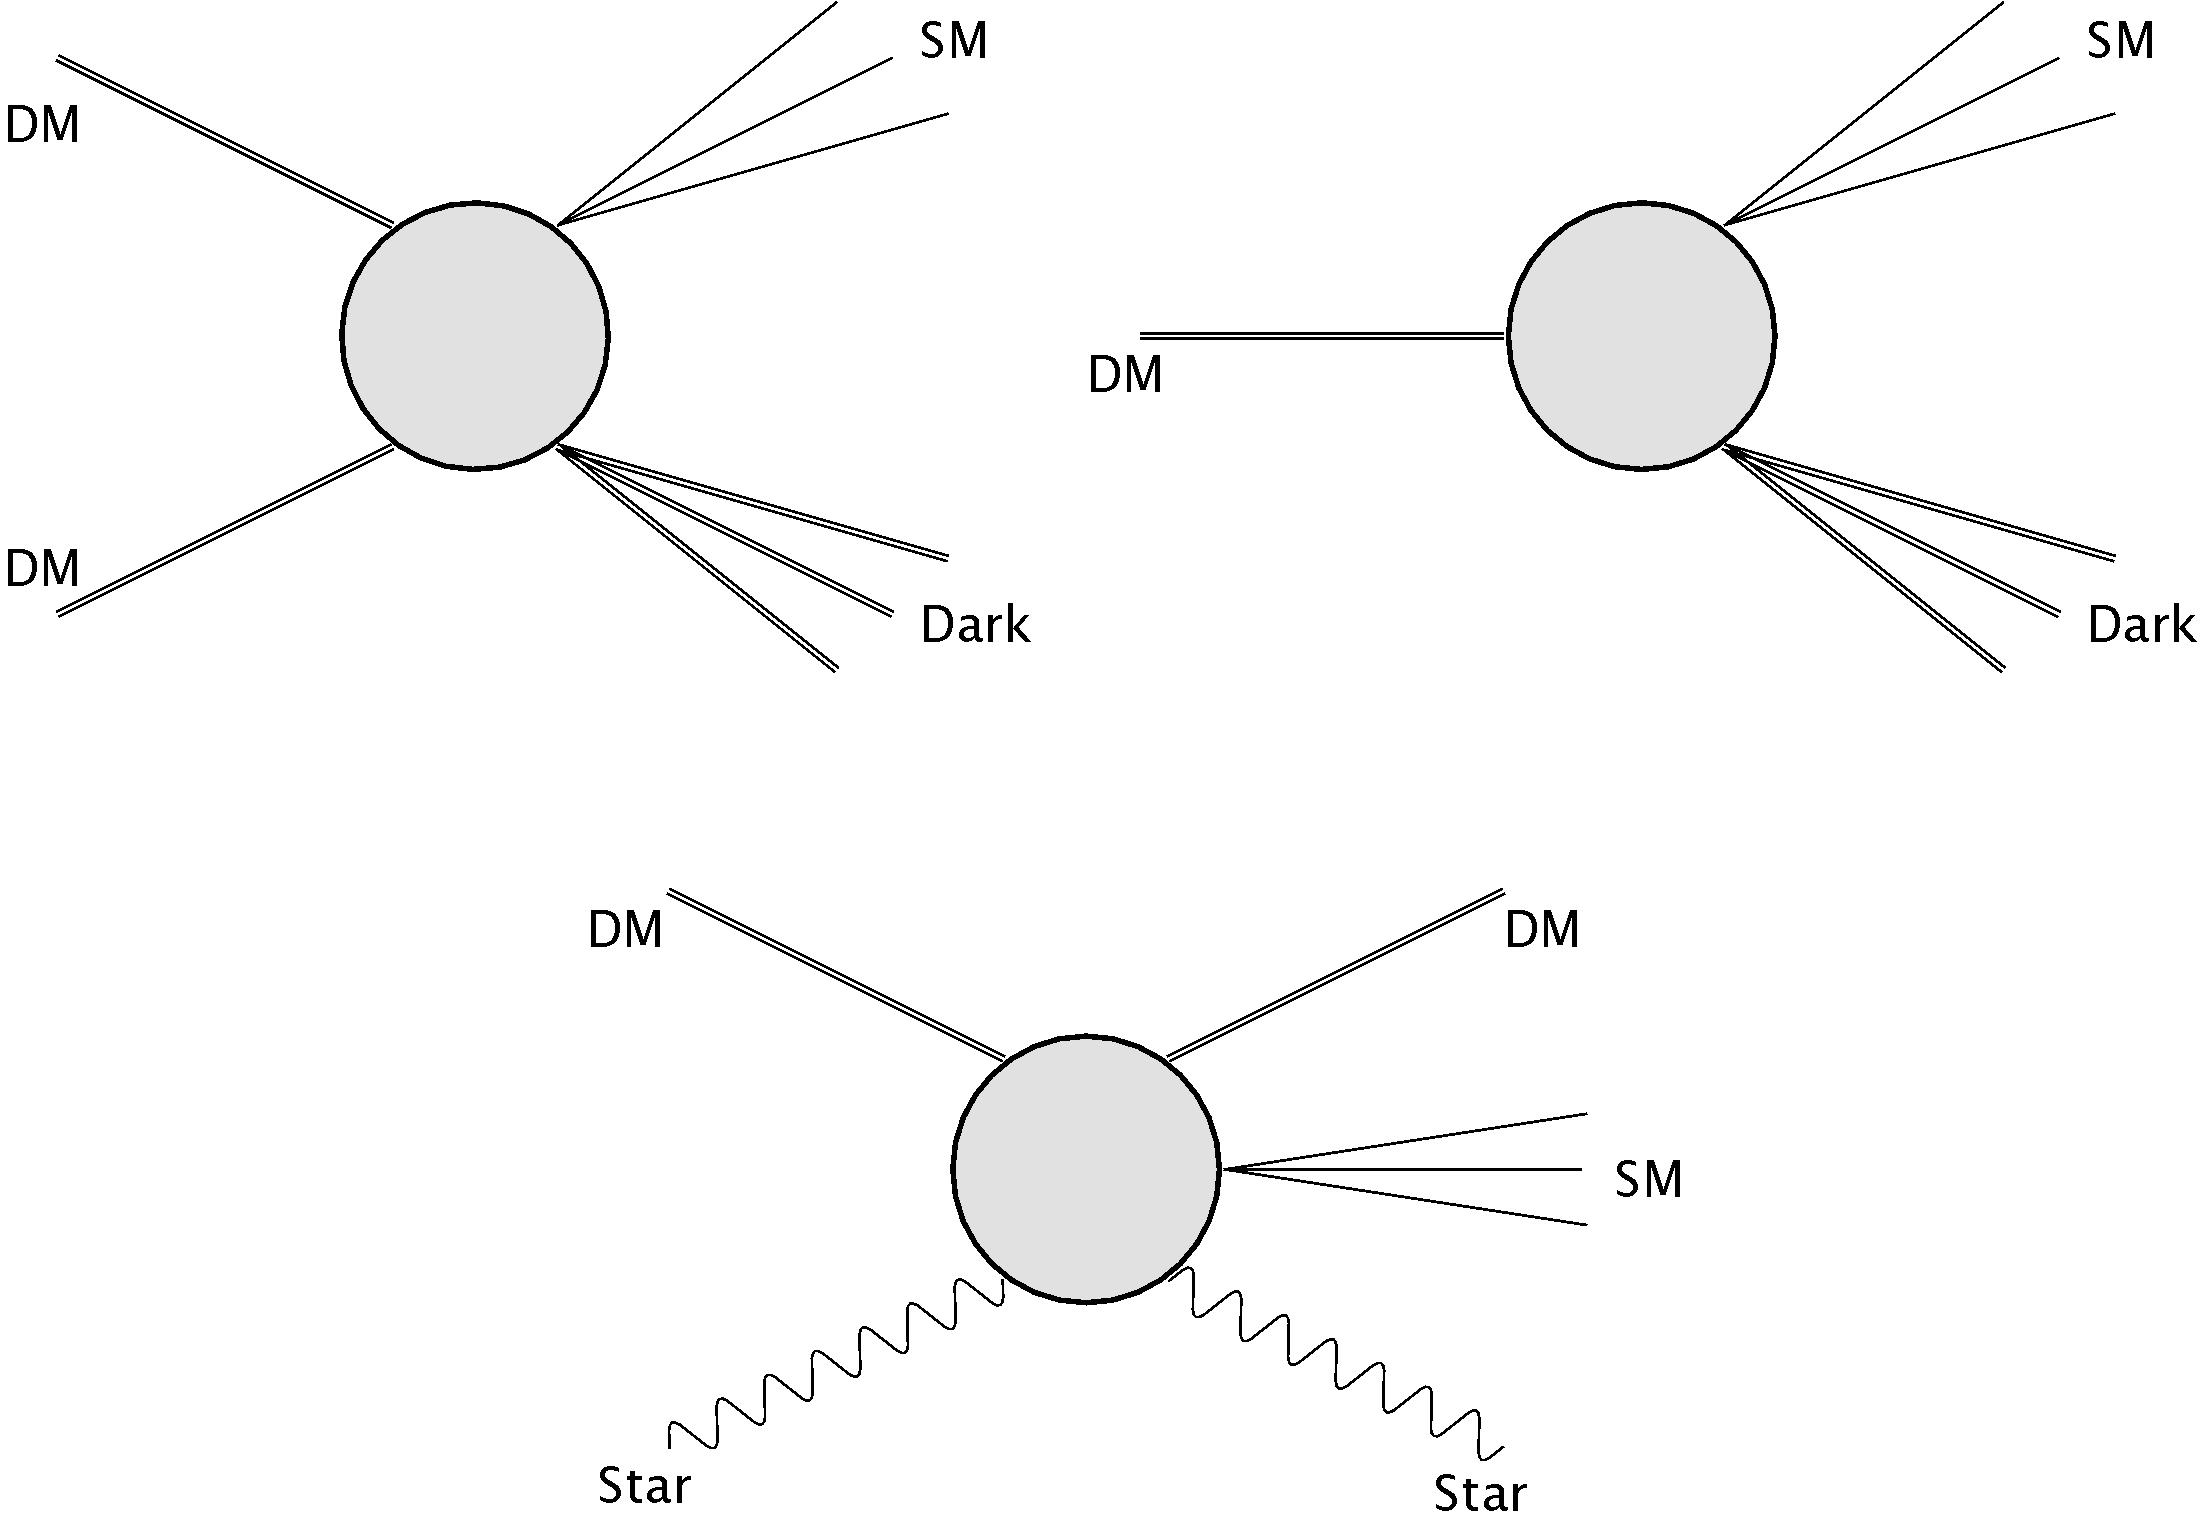
\includegraphics[scale=.05]{feynmandiag}
\caption{General interactions between ultra-heavy DM and WD constituents - \textcolor{blue}{do diagrams properly}}
\label{fig:feynman}
\end{figure}

\subsection{DM-DM Collisions and DM Decays}
\label{sec:coldecay}
In this section, we consider the collision of two DM particles or the decay of a single DM particle into a SM secondaries within the WD.  Note that these DM-DM collisions are not necessarily particle-antiparticle annihilations, but can be of a more general, complicated nature, such as the collisions of heavy nuclei.  For simplicity, we restrict our attention to point-like events, where the SM products are produced near enough to the initial collision or decay event to give rise to a single temperature peak.  This excludes ``displaced vertex" events, whose explosion conditions would involve additional model-dependent parameters.  

With this restriction, the explosion condition depends only on the total energy released into SM particles and the heating length $L_0$ of the SM products.  Since the DM involved in this process is non-relativistic, the available energy for SM products is $\sim m_\text{DM}$ and we parameterize the energy released in the SM as a fraction $\eta$ of the DM mass.  The explosion condition is:
\begin{equation}
\label{eq:coldecay}
    m_\text{DM} \gtrsim n_\text{ion} T_f \lambda_T^3 \cdot \frac{1}{\eta}
      \text{max}\left\{1, \frac{L_0}{\lambda_T}\right\}^3
\end{equation}
Considering the explosion threshold \eqref{eq:Eboom}, this process necessarily requires ultra-heavy DM $m_\text{DM} \gtrsim 10^{14} ~\GeV$. 

\subsection{DM Transit}
\label{sec:transit}
For models with a DM-SM scattering process as in Figure \ref{fig:feynman}, there will be a continuous production of SM particles as the DM traverses a WD.  We consider a \emph{transit} to be the special case of a DM state that loses only a small fraction of its kinetic energy to the star during this process, so that we may ignore any perturbations to the DM trajectory. More precisely, any DM model will have a \emph{stopping power} $d E_\text{DM}/d x$ with the WD medium, which is the kinetic energy lost by the DM per distance traveled.  For a transit to occur, we require that
\begin{align}
\frac{d E_\text{DM}}{d x} \lesssim \frac{m_\text{DM} v^2_\text{esc}}{R_\text{crust}},
\label{eq:CrustCondition}
\end{align}
where $R_\text{crust} \sim \text{km}$ \textcolor{red}{check this} is the width of the non-degenerate WD crust, and $v_\text{esc}$ is the escape velocity of the WD. Note that we have conservatively estimated the crust density to be $\OO(1)$ of the interior density. It is crucial that a transiting DM penetrate the crust as it is only in the degenerate WD interior that runaway fusion can occur.  If \eqref{eq:CrustCondition} were violated, we would have to account for possible variations in the kinematic state of the DM after traversing the crust for various stopping powers. Furthermore, since $R_\text{crust}$ will ultimately be larger than any of the heating lengths considered, \eqref{eq:CrustCondition} ensures that there is negligible variation in the DM trajectory through a heating region as well. 

The ability of a transit to ignite the star is most generally parameterized by a \emph{linear energy transfer} (LET) $d E_\text{SM}/d x$, which is the energy released into thermalizing SM products per distance traveled. Note that the LET and stopping power are in fact equal in the special case that the DM-SM interaction converts only DM kinetic energy into SM particles. However, these two model-dependent parameters will generically be quite different. For instance, such a scenario occurs if most of the released energy is due to changes in mass, as is the case for the interaction of Q-ball DM considered in Section \ref{sec:ConcreteExamples}. 

In order to ignite a WD during transit, the energy released must exceed the threshold \eqref{eq:boom}.  If the heating length $L_0$ of the SM products is larger than the trigger size, we consider one segment $L_0$ of the transit which behaves as a single energy deposit of size $L_0$ as described in Section \ref{sec:Review}. However, if $L_0 < \lambda_T$ then many small-scale heating events will overlap during a transit segment of length $\lambda_T$ as they diffuse outward and sum to give a temperature peak over the entire $\lambda_T$ sized region. Combining these gives the the explosion condition for transits
\begin{equation}
\label{eq:transitexplosion}
  \frac{d E_\text{SM}}{d x} \gtrsim n_\text{ion} T_f\, \text{max}\left\{\lambda_T, L_0 \right\}^2
\end{equation}

Note that condition \eqref{eq:transitexplosion} has been derived by adding the energy deposited along a length $\text{max} \{L_0, \lambda_T\}$ to produce a net energy deposit.  This is only valid if the timescale for heat to diffuse out to this distance is larger than the timescale over which the energy is deposited into the medium, i.e. the DM transit time:
\begin{equation}
\tau_d \gtrsim \frac{\text{max}\left\{ \lambda_T, L \right\}}{v_\text{esc}},
\end{equation}
where the DM transit velocity is given by the WD escape velocity and $\tau_d$ is the characteristic time for a region of size $\text{max}\{\lambda_T, L\}$ and temperature $T_0 \sim \mathcal{E}_0 / n_\text{ion} \text{max}\{\lambda_T, L\}^3$ to diffuse $\OO(1)$ of its thermal energy.  According to the heat equation, this scales as $\tau_d \sim \text{max}\left\{ \lambda_T, L \right\}^2/\alpha$, where $\alpha$ is the temperature-dependent diffusivity. Thus, we require:
\begin{equation}
\alpha (T_0) \lesssim v_\text{esc} \text{max}\left\{ \lambda_T, L \right\} 
\label{eq:SlowDiffusion}
\end{equation}
This condition is independent of DM model, and is satisfied for all WD densities. 
\textcolor{red}{Show this is actually true for all densities.} \textcolor{red}{There is some subtlety here, as $\alpha$ should increase with $T$. But we also do not need to consider arbitrary large $T$, as for large enough $T$ the runaway will occur even if we don't sum the profiles. Need to work this out. It would probably be useful in general to understand the $T$ dependence of $\alpha$.}

\section{Heating Length}
\label{sec:HeatingLength}
A heating event in the WD must efficiently transfer energy to ions in order to trigger runaway fusion, as concisely stated in \eqref{eq:runaway}. With regards to the processes described in Section \ref{sec:DMexplode}, the characteristic heating length $L_0$ depends on the exact nature of the DM interaction and must be explicitly calculated for a given DM model to determine its explosiveness \eqref{eq:transitexplosion}. However, any such calculation necessarily involves an understanding of how individual SM particles dump their energy to the stellar medium. In this section, we summarize the stopping powers for particles interacting via the strong and electromagnetic forces in a WD - a detailed analysis of the energy loss is given in Appendix \ref{sec:appendix}. We define $L_i(\epsilon)$ as the distance over which an incident particle $i$ of energy $\epsilon$ (and any secondaries) deposits $\OO(1)$ of the initial energy to the stellar medium \emph{and} thermalizes ions. This length scale is calculated in the case of incident hadrons, electrons, and photons. As we are only concerned with depositing sufficient energy to ignite supernovae, we restrict our attention to high-energy particles $\epsilon \gg T_f \sim \text{MeV}$. As such, the WD may be thought of as a ``particle detector" with electromagnetic and hadronic ``calorimeter" components.

\subsection{Hadrons}
\textcolor{blue}{Orange = Coulomb off electrons, Blue = Coulomb off Ions, Magenta = Nonelastic Nuclear, Green = Elastic Nuclear.}
The stopping powers for incident nucleons (protons, neutrons) and pions in a WD are depicted in Figures \ref{fig:SPnuc} and \ref{fig:SPpion}. Note that the energy loss due to Coulomb collisions is only applicable for incident charged particles. At energies greater than the typical nuclear binding energy $\epsilon \gtrsim 10 ~\text{MeV}$, the energy loss is dominated by nonelastic nuclear collisions in which secondary hadrons carry the initial energy in a roughly collinear shower. As shown in Appendix \ref{sec:appendix}, the total hadronic shower length is given by
\begin{equation}
X_{\text{had}} \sim l_\text{had} \log{(\epsilon/E_c)} \approx 10 ~l_\text{had},
\label{eq:hadlength}
\end{equation}
where $E_c \sim 10 ~\text{MeV}$ as there are no other dominant stopping mechanisms above the nuclear binding energy, and $l_\text{had}$ is the mean free path for nonelastic scatters. Therefore after a distance $X_\text{had}$, the initial energy is approximately completely contained in an exponential number of final-state hadrons of energy $1 - 10 ~\text{MeV}$. At this stage, hadrons will predominantly transfer energy to nuclei via nuclear elastic scatters. For neutrons and protons $N \sim 10$ collisions are needed to transfer an $\OO(1)$ fraction of this energy while for pions, $N \sim 100$ collisions are needed. This will be in the form of a random walk $X_\text{elastic} = l_\text{el} \sqrt{N}$, where $ l_\text{el} = 1/n_\text{ion} \sigma_\text{el}$ is the mean free path for elastic scatters. We find that $L_\text{hadron} \approx X_\text{had} + X_\text{el}$ is dominated by the size of the hadronic shower \eqref{eq:hadlength} as opposed to the final deposition length. As a result, $L_\text{hadron}$ scales roughly linearly in WD density. This is plotted in Figure \ref{fig:cash} for the maximal WD density $n_e \sim 10^{33} ~\text{cm}^{-3}$. 

\begin{figure}
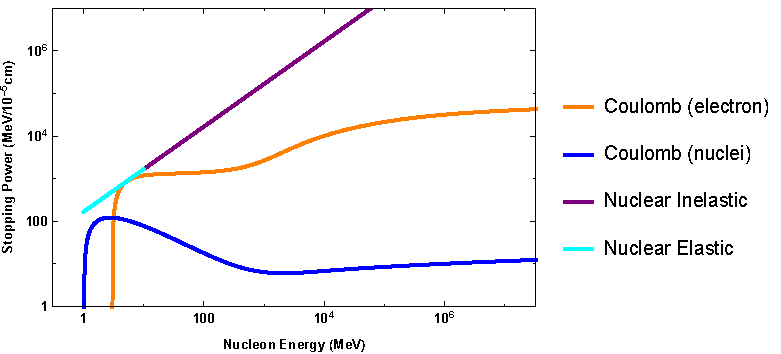
\includegraphics[scale=.45]{SPnucleon.pdf}
\caption{Nucleon energy loss in a WD density $n_e = 10^{33} ~\text{cm}^{-3}$.}
\label{fig:SPnuc}
\end{figure}

\begin{figure}
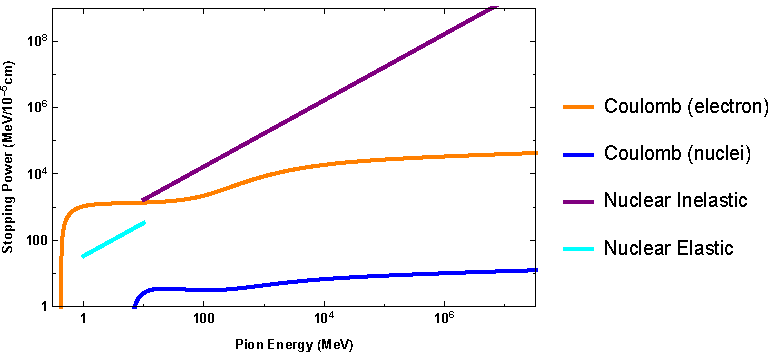
\includegraphics[scale=.45]{SPpion.pdf}
\caption{Pion energy loss in a WD density $n_e = 10^{33} ~\text{cm}^{-3}$.}
\label{fig:SPpion}
\end{figure}

\subsection{Electrons and Photons}

The stopping power of electrons and photons is highly sensitive to the density of the stellar medium. This is evident in the fact that there is a critical density $n_e \sim 10^{32} ~\text{cm}^{-3}$ above which bremsstrahlung and pair production can essentially be ignored. We begin by considering WD densities $n_e \lesssim 10^{32} ~\text{cm}^{-3}$. The electron and photon energy loss functions for a characteristic density in this range are shown in Figures \ref{fig:SPelectron} and \ref{fig:SPphoton}. For both species, the dominant stopping mechanism at incident energies $\epsilon \sim 10^{3}-10^{5} ~\text{MeV}$ is due to electromagnetic radiative processes. For an incident electron or photon of energy $\epsilon$, this will result in a cascade of secondary electrons and photons with typical shower length
\begin{equation}
X_\text{em} \sim \frac{2}{X_0} \l \l \frac{\epsilon}{E_\text{LPM}}\r^{1/2} - \l \frac{E_c}{E_\text{LPM}}\r^{1/2} \r,
\end{equation}
where $X_0$ is the radiation length and $E_\text{LPM}$ is the typical scale of LPM suppression, defined in Appendix \ref{sec:appendix}. In the electromagnetic case, $E_c \sim ~\text{TeV}$ is set by the energy at which Compton scattering dominates the stopping power and is thus the process which terminates shower propagation. At $\epsilon \sim 10^{5} ~\text{MeV}$, bremsstrahlung is suppressed by $\OO(\alpha)$ due to the LPM effect \textcolor{blue}{how do we treat this?}. 

Therefore, at sufficiently high energies $\epsilon \gtrsim 10^5 ~\text{MeV}$ electrons and photons in the WD will lose energy primarily through nuclear interactions. Effectively, electrons and photons at this energy behave like hadrons and will dump an $\OO(1)$ fraction of their initial energy into hadronic showers of length \eqref{eq:hadlength}. However, the initial distance traversed to trigger a hadronic shower will vary between the two species. For photons, this is roughly the photonuclear mean free path $l_\gamma$ while for electrons, the ``electronuclear radiation length" is found to be of order $\sim 10  ~l_\gamma/\alpha$. Note that these initial length scales will dominate the overall size of $L_i$ as compared to the hadronic shower length. In addition, $L_\text{electron}$ and $L_\text{photon}$ in this energy range also scale roughly linearly with WD density. We now consider $n_e \gtrsim 10^{32} ~\text{cm}^{-3}$, for which radiative processes are negligible. In this density regime, the stopping of electrons of incident energy $\epsilon \sim 1 - 10^4 ~\text{MeV}$ is primarily due to Coulomb collisions off degenerate electrons in the star. At energies $\epsilon \gtrsim 10^4 ~\text{MeV}$, electronuclear and photonuclear processes become the dominant source of energy loss. 

\begin{figure}
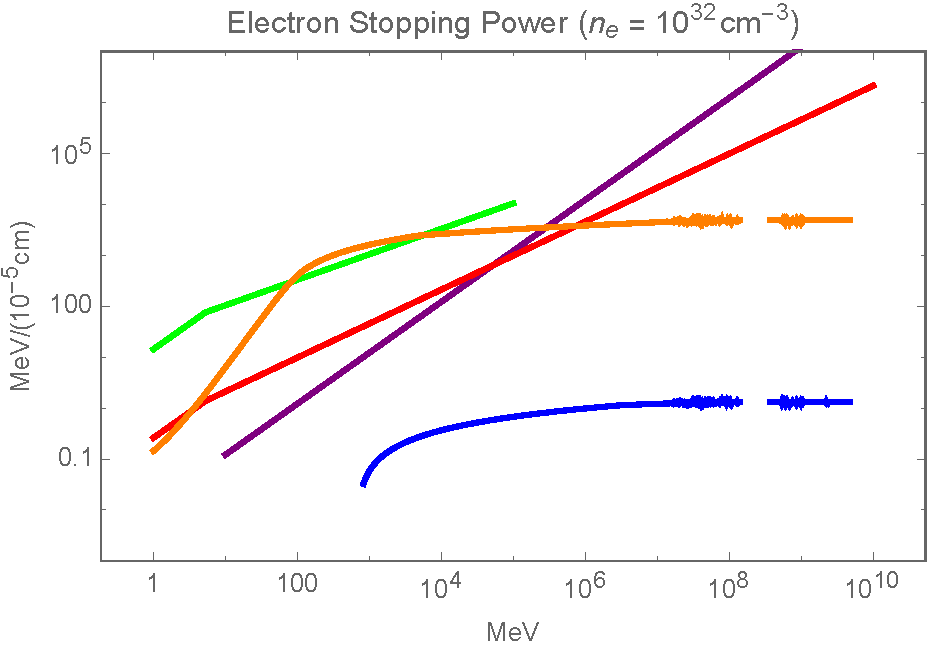
\includegraphics[scale=.45]{SPelectron.pdf}
\caption{Electron energy loss in a WD density $n_e = 10^{32} ~\text{cm}^{-3}$}
\label{fig:SPelectron}
\end{figure}

\begin{figure}
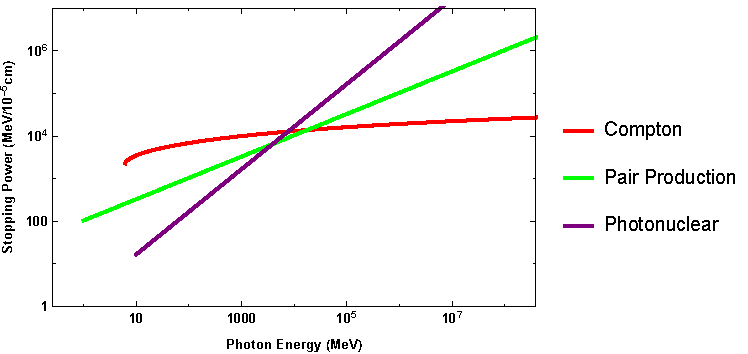
\includegraphics[scale=.45]{SPphoton.pdf}
\caption{Photon energy loss in a WD density $n_e = 10^{32} ~\text{cm}^{-3}$}
\label{fig:SPphoton}
\end{figure}

\begin{figure}
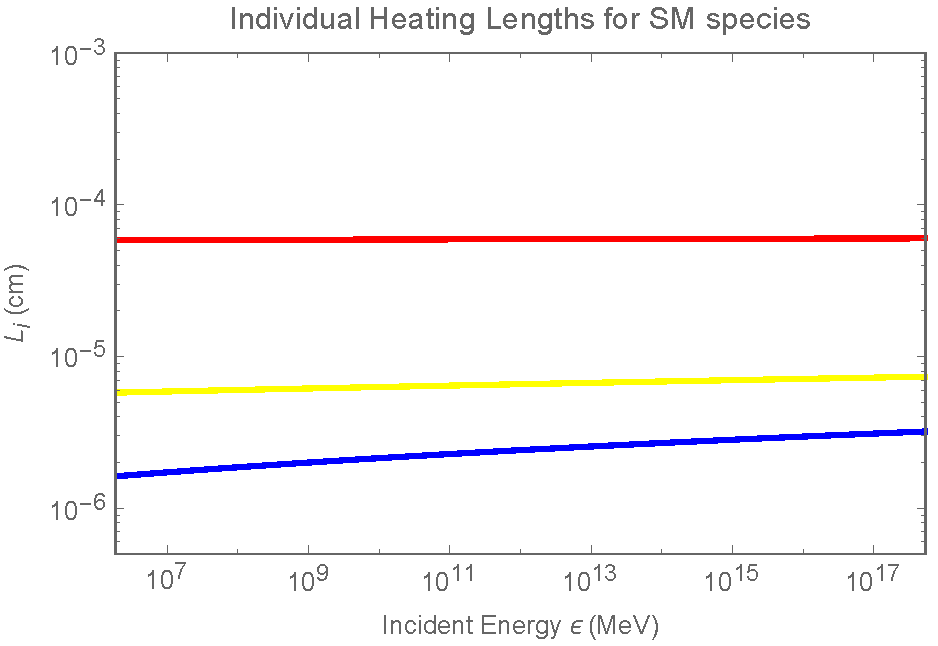
\includegraphics[scale=.45]{cashmoney.pdf}
\caption{$L_i (\epsilon)$ computed for incident electrons, photons, and hadrons in a WD of density $n_e \sim 10^{33} ~\text{cm}^{-3}$. \textcolor{blue}{Blue = Hadrons, Yellow = Photons, Red = Electrons}}
\label{fig:cash}
\end{figure}


\section{Constraints}
\label{sec:Constraints}

In this section, we constrain generic ultra-heavy DM models that can interact with a WD to trigger supernova. Following the discussion of \cite{Graham:2015apa}, these constraints will come from (1)~the existence of long-lived white dwarfs and (2)~the measured type Ia supernovae rate. In particular, both (1) and (2) will be affected if the DM of the universe were capable of igniting WDs via one the processes described in Section \ref{sec:DMexplode}. We will consider both classes of observations, but first we review relevant data available on white dwarfs and the supernovae rate.

RX~J0648.04418 is one of the heaviest known white dwarfs with a mass $M = 1.28\pm 0.05 ~M_{\odot}$. Using a digitization of the WD mass-radius relation, we find that $R \approx 3000~\text{km}$ so that the stellar escape velocity $v_\text{esc} \approx 4 \times 10^{-2}$. \textcolor{blue}{this is likely a carbon WD (SR), but not sure...} Note that RX~J0648.04418 is not the only known heavy WD (Sloan Digital Sky Survey has found $\sim 20$ others - see \href{https://heasarc.gsfc.nasa.gov/db-perl/W3Browse/w3hdprods.pl}{survey}).

\textcolor{blue}{discuss SN rate}

\subsection{Transit Constraints}
\label{sec:TransitConstraints}

For a DM candidate to be constrained through its transit interaction with a WD, we demand that it penetrate the crust \eqref{eq:CrustCondition}, satisfy the explosive condition \eqref{eq:transitexplosion}, and have sufficient abundance that a single transit is expected to occur during the lifetime of the observed star. The lattermost condition can be viewed as a ``flux is too low" fundamental limit for the WD as a DM detector. 

The expected number of DM transits through a WD with lifetime $t_\text{WD} \sim \text{Gyr}$ is given by
\begin{align}
N_\text{transits}  &= t_\text{WD} \cdot n_\text{DM} \sigma_g v \nonumber\\
 &  \sim t_\text{WD} \cdot \frac{\rho_{\text{DM}}}{m_\text{DM}} \pi R_\text{WD}^2 \l\frac{v_\text{esc}}{v}\r^2 v. 
\label{eq:TransitFluxCondition}
\end{align}
where $v \sim 10^{-3}$ is the DM virial velocity \textcolor{red}{different for galactic center?}, and $\rho_{\text{DM}}$ is the energy density of DM in the region of interest. $\sigma_g$ denotes the capture cross section including a gravitational Sommerfeld enhancement. Considering a $1.2 ~M_{\odot}$ WD in the local dark matter halo $\rho_{\text{DM}} \sim 0.4~\text{GeV}/\text{cm}^3$ such as RX~J0648.04418, we find that $m_\text{DM} \lesssim 10^{44} ~\GeV \sim 10^{20} ~\text{g}$ will transit the star at least once in a Gyr. If we instead consider recently discovered $\sim 1.2 ~M_{\odot}$ WDs in the galactic center \textcolor{blue}{NuStar} where $\rho_{\text{DM}} \sim 10^3 ~\text{GeV}/\text{cm}^3$, this upper bound improves to $m_\text{DM} \lesssim 10^{48} ~\GeV \sim 10^{24} ~\text{g}$. \textcolor{blue}{matches what SR found}

As shown in Section \ref{sec:DMexplode}, a general DM transit is described by a stopping power $d E_\text{DM}/dx$ and LET rate $dE_\text{SM} /dx$. The former parameterizes the extent to which the DM slows down in the WD by losing kinetic energy, while the latter parameterizes the ability for the DM to dump sufficient energy to the star in the form of SM particles. Let $\sigma_{i,\epsilon}$ denote the cross section for DM to scatter off a stellar constituent (ion or electron), producing a single SM particles of species $i$ and energy $\epsilon$. If this were the only available channel for the DM to deposit energy, then the LET rate could be written as
\begin{equation}
\label{eq:schematicLET}
\frac{d E_\text{SM}}{d x} = n_\text{ion} \sigma_{i,\epsilon} \epsilon,
\end{equation}
where we have now specified to DM interactions with nuclei in the WD. Of course, the LET rate for any realistic DM model would necessarily involve a sum over species $i$ (of variable number) that could be produced as well as an integral over their spectrum. For simplicity, we will assume a schematic picture in which \eqref{eq:schematicLET} adequately describes the DM transit through a WD. The heating length of any such interaction is simply $L_i$ for each produced species of energy $\epsilon$, which was explicitly calculated in Section \ref{sec:HeatingLength} for hadrons, electrons and photons. As an example, an interaction with $i = \text{photon}$ and $\epsilon = \GeV$ would describe DM transferring energy to the stellar medium solely via the production of one $\GeV$ photon per nuclear collision. In addition, we make a sensible assumption that the stopping power and LET are related in a straightforward manner - the DM loses kinetic energy at the same rate as energy is deposited to the WD as per the LET. As a result, condition \eqref{eq:CrustCondition} takes the form
\begin{equation}
\label{eq:schematicCrust}
\sigma_{i,\epsilon} \epsilon \lesssim \frac{m_\text{DM}v_\text{esc}^2}{n_\text{ion} R_\text{crust}}.
\end{equation}
While such a statement is certainly not true for all DM models (such as the Q-ball), it provides a useful benchmark to express constraints. It is interesting to note that combining \eqref{eq:schematicLET} and \eqref{eq:schematicCrust} with the transit explosion condition \eqref{eq:transitexplosion}, we find a lower bound on $m_{\text{DM}}$ such that the DM is able to both penetrate the crust \emph{and} trigger an explosion:
\begin{equation}
\label{eq:transitmass}
m_{\text{DM}} \gtrsim  T_f ~\text{max}\{\lambda_T, L\}^2 \l \frac{n_{\text{ion}} R_{\text{crust}}}{v_{\text{esc}}^2} \r
\end{equation}
In other words, if \eqref{eq:transitmass} were violated then the DM interaction is either not strong enough to ignite the WD or it is so strong that it has no chance to penetrate the crust and transit the interior. In the case of $\lambda_T > L_0$, this translates to a lower-bound on the DM mass $\sim 10^{27} - 10^{34} ~\GeV$.

Within this schematic for the DM-WD interaction, one can constrain the parameter $\sigma_{i,\epsilon} \epsilon$ as a function of DM mass $m_\text{DM}$. Note that this limit can be placed over a range of produced energies $\epsilon \sim 10^{6} - 10^{18} ~\text{MeV}$ using the values of $L_i (\epsilon)$ calculated in Section \ref{sec:HeatingLength}. As an example, this is done for released photons and electrons in Figures \ref{fig:photonconstraint} and \ref{fig:electron} for a WD of mass $\sim 1.25 M_\odot$.
\begin{figure}
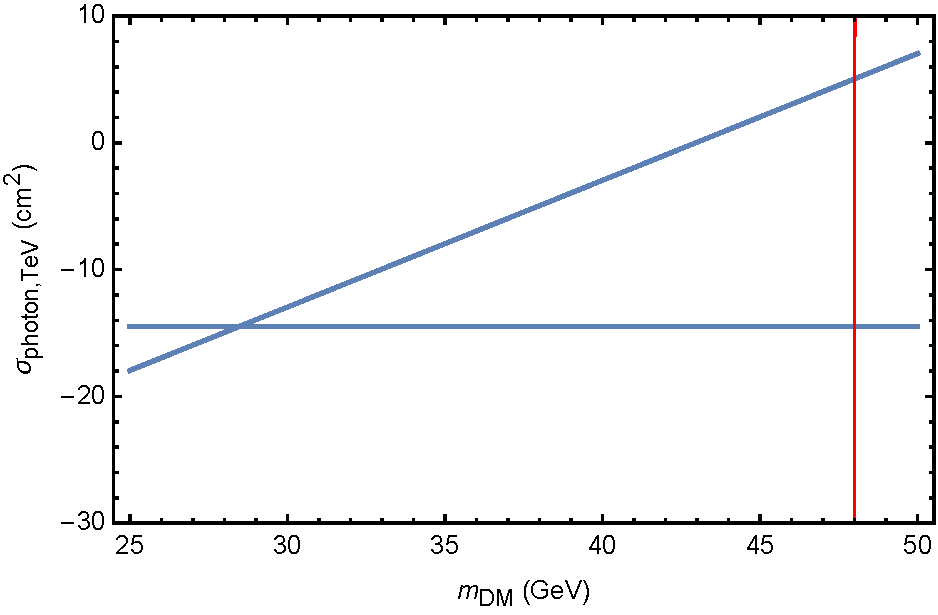
\includegraphics[scale=.45]{photonconstraint.pdf}
\caption{\textcolor{blue}{Photons produced at $\epsilon = \text{TeV}$, constraint is region enclosed by three curves}}
\label{fig:photonconstraint}
\end{figure}
\textcolor{blue}{Electron plot looks nearly the same - only difference is in $L_i$, so maybe no need to show for different species?}. 

\subsection{DM-DM Collision Constraints}
\label{sec:CollisionConstraints}

In the case of the collision of two dark matter particles, we find more stringent upper bound on the masses which will produce at least one event per Gyr in a given white dwarf. The expected number of collisions in a white dwarf within its lifetime is
\begin{align}
N_\text{collisions}  &= t_\text{WD} \cdot n_\text{DM}' \sigma_\text{DM-DM} v \cdot n_\text{DM}'R_\text{WD}^3
\end{align}
\textcolor{red}{revisit this}
where $n'_\text{DM}$ is the gravitationally enhanced dark matter density within the star.


\subsection{DM Decay Constraints}
\label{sec:DecayConstraints}




\section{Q-balls}
\label{sec:ConcreteExamples}

We now implement the formalism for general constraints outlined in Section \ref{sec:Constraints} to place bounds on a specific model of DM: Q-balls. In various supersymmetric extensions of the SM, non-topological solitons called Q-balls can be produced in the early universe \cite{Coleman:1985ki, Kusenko:1997si}. If these Q-balls were stable, they would comprise a component of the DM today.

In gauge-mediated models with flat scalar potentials, the Q-ball mass and radius are given by
\begin{equation}
\label{eq:Qballprop}
M_Q \sim m_S Q^{3/4}, ~~~ R_Q \sim m_S^{-1} Q^{1/4},
\end{equation}
where $m_S$ is related to the scale of supersymmetry breaking. The condition $M_Q/Q < m_p$ ensures that the Q-ball is stable against decay to nucleons \cite{Dine:2003ax}. When an (electrically neutral) baryonic Q-ball interacts with a nucleon, it absorbs its baryonic charge as a minimum-energy configuration and induces the dissociation of the nucleon into free quarks. During this process, $\sim \text{GeV}$ of energy is released through the emission of 2-3 pions \cite{Dine:2003ax}. We assume that for each Q-ball collision, there is equal probability to produce $\pi^0, \pi^+$ and $\pi^-$ under the constraint of charge conservation. The cross section for this interaction is approximately geometric:
\begin{equation}
\sigma_Q \simeq \pi R_Q^2.
\end{equation}
Note that a sufficiently massive Q-ball will become a black hole if the Q-ball radius is less than the Schwarzschild radius $R_Q \lesssim R_s \sim G M_Q$. In the model described above, this translates into a condition
\begin{equation}
m_S \l\frac{\Mpl}{m_S}\r^3 \lesssim m_Q, ~~~ \l\frac{\Mpl}{m_S}\r^4 \lesssim Q.
\end{equation}
For Q-ball masses of this order, gravitational interactions become relevant.

We now summarize the explosiveness of a Q-ball transit. According to the notation of Section \ref{sec:Constraints}, the Q-ball transit is parameterized by 
\begin{equation}
\frac{d E_\text{SM}}{d x} = N_\pi \cdot n_\text{ion} \sigma_Q \epsilon,
\end{equation}
where the nuclear interaction results in $N_\pi \sim 30$ pions released, each with kinetic energy $\epsilon \sim 500 ~\text{MeV}$. Numerous experiments have studied interactions of pions in this energy range incident upon complex nuclei targets such as carbon. It is found that there is roughly equal cross section of order $\OO (100 ~\text{mb})$ for a (neutral or charged) pion to either elastically scatter or become absorbed in a nonelastic scatter with no final state pion \cite{Pionnuclear}. As seen in Section \ref{sec:HeatingLength}, nonelastic collisions are most relevant for energy loss and will induce a hadronic shower. The corresponding heating length of the Q-ball interaction is computed in a straightforward manner
\begin{equation}
L_0^\text{Q-ball} \sim \text{few} \times 10^{-7} ~\text{cm}
\end{equation}
in WD density of $n_\text{ion} \sim 10^{32} ~\text{cm}^{-3}$. The resulting explosiveness of the Q-ball transit as a function of WD mass is plotted in Figure \ref{fig:boomQball}. 
\begin{figure}
\label{fig:boomQball}
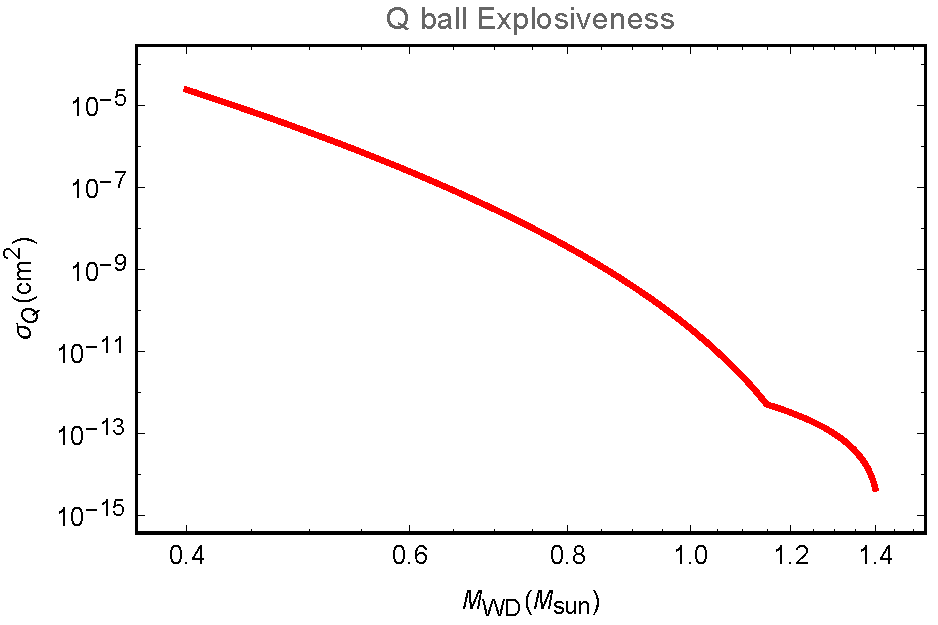
\includegraphics[scale=.45]{boomQball.pdf}
\end{figure}
If the Q-ball cross section is related to its mass and baryonic charge as in \eqref{eq:Qballprop}, we find that
\begin{equation}
\label{eq:Qballbound}
m_Q \gtrsim 10^8 ~\text{g} \l\frac{m_S}{\text{TeV}}\r^4, ~~~~ Q \gtrsim 10^{38} \l\frac{m_S}{\text{TeV}}\r^4
\end{equation}
is capable of triggering runaway fusion in a heavy $\sim 1.25 ~M_{\odot}$ WD. Note that for such large values of $Q$ there is negligible stopping power for the Q-ball to slow down in a WD, and as such condition \eqref{eq:CrustCondition} will be trivially satisfied. 

Combining \eqref{eq:Qballbound} with the model-independent limits derived in Section \ref{sec:Constraints}, we find that Q-ball DM of mass $10^{8} - 10^{20} ~\text{g}$ is ruled out and perhaps $10^{8} - 10^{24} ~\text{g}$ is under constrain \textcolor{blue}{if you trust the NuStar results}. We can make these constraints more robust by comparing the effectiveness of the WD detector with other bounds on Q-ball DM. Currently, the most stringent constraints on Q-balls come from air fluorescence detectors of cosmic rays (OA, TA) as well as the Super-Kamiokande Cherenkov detector. However, the constraints possible through WD observation are in a fundamentally inaccessible region of parameter space for these terrestrial-based experiments. This is shown in Figure \ref{fig:Qballconstraint}

\begin{figure}
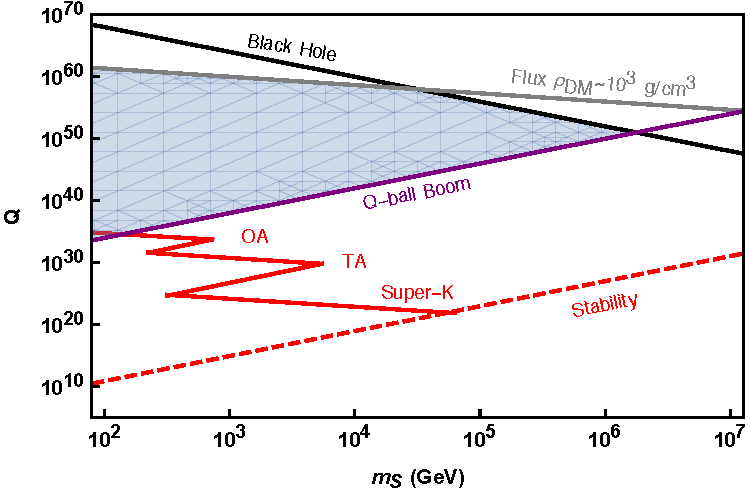
\includegraphics[scale=.45]{Qballconstraint.pdf}
\caption{Constraints on baryonic Q-balls. \textcolor{blue}{Black = stability line, Cyan = Super-K, Green = OA + TA, Blue dashed = boom, Red dashed = Flux too low, Black dashed = Q-ball becomes Black hole.}}
\label{fig:Qballconstraint}
\end{figure}

\section{Discussion}
\label{sec:discussion}

\begin{appendices}

\section{Particle Interactions in a White Dwarf}
\label{sec:appendix}

The interior of a WD is a complex environment (unless otherwise noted, we will assume a carbon-oxygen WD). Famously, the star is supported against collapse by electron degeneracy pressure with a characteristic Fermi energy
\begin{equation}
E_F = (3 \pi^2 n_e)^{1/3} \sim 0.1 - 1 ~\text{MeV}
\end{equation}
where $n_e$ is the number density of electrons. The nuclei are at an ambient temperature $T \sim \text{keV}$ and form a strongly-coupled plasma with coupling parameter
\begin{equation}
\Gamma \sim \frac{Z^2 \alpha}{n_\text{ion}^{-1/3} T} \gg 1,
\end{equation}
where $n_\text{ion}$ is the number density of nuclei. Here we provide a detailed analysis of the possible electromagnetic and strong interactions in a WD.

\subsection*{Coulomb Collisions}

An incident particle of mass $m$, charge $e$, and velocity $\beta$ scattering off a (stationary) target of mass $M$, charge $Ze$ with impact parameter $b$ will transfer energy
\begin{equation}
\label{eq:impact}
E' = \frac{2 Z^2 \alpha^2}{b^2 \beta ^2 M}.
\end{equation}
The differential cross section for the interaction is given by the Rutherford cross section
\begin{equation}
\label{eq:rutherford}
\frac{d \sigma_R}{dE'} = \frac{2 \pi  \alpha^2 Z^2}{M \beta^2} \frac{1}{E'^2},
 \end{equation}
where we have assumed a sufficiently fast incident particle so that interactions are governed by single collisions with energy transfer $E'$ \cite{Agashe:2014kda}.  Note that the differential cross section receives additional QED due to the incident spin, but for small energy transfers these corrections are negligible. It is straightforward to understand the parametric dependences of \eqref{eq:rutherford}: there is increased likelihood to scatter for slowly moving incident particles undergoing ``soft-scatters" against lighter targets. Therefore, one would expect that soft-scattering dominates the energy loss and that collisions with nuclei of mass $M$ are suppressed by a factor $\OO\l\frac{Z m_e}{M}\r$ as compared to collisions with electrons. This is certainly true for incident charged particles in non-degenerate matter. However, both of these naive expectations turn out to be false when considering scattering off a degenerate species.

We first consider the energy loss of high-energy charged particles colliding with non-degenerate targets. In this case, the stopping power is given by:
\begin{align}
\label{eq:SP}
-\l \frac{dE}{dx}\r_\text{coulomb} & = - \int dE' \left(\frac{d \sigma}{dE'}\right) n E' \\
& \simeq -\frac{n_\text{ion} \pi Z^2 \alpha^2}{M \beta^2} \log {\l\frac{E_{\text{max}}}{E_{\text{min}}}\r}.
\end{align}
\eqref{eq:SP} must be integrated over all $E'$ within the regime of validity for \eqref{eq:rutherford}, thereby fixing the lower and upper bounds of the Coulomb logarithm. The maximum possible energy transfer satisfying kinematic constraints in a backward scatter is given by
\begin{equation}
E_{\text{kin}} = \frac{2 M \beta^2 \gamma^2}{1+ 2\gamma M/m +(M/m)^2},
\end{equation}
where $\gamma = (1-\beta^2)^{-1/2}$ is the relativistic factor. In addition, quantum mechanical uncertainty sets a limit to the accuracy that can be achieved in ``aiming" an incident particle at a target $b > \frac{1}{\text{min}\{{M, m}\} \beta \gamma}$. In terms of energy transfer, this translates to the condition
\begin{equation}
E' < E_\text{quant} = \frac{2 Z^2 \alpha^2 \gamma^2 ~\text{min}\{{M, m}\}^2}{M}.
\end{equation}
Furthermore, the expression for the energy loss in a scatter \eqref{eq:impact} is modified by relativistic considerations when the energy transfer is larger than the target mass \cite{Rossi}. For our purposes, we take the maximum energy that an incident particle is able to transfer to be
\begin{equation}
E_{\text{max}} = \text{min}\{E_\text{quant}, E_{\text{kin}}, M\}.
\end{equation}

On the other hand, the maximum impact parameter is set by Thomas-Fermi screening due to the degenerate electron gas:
\begin{equation}
\label{eq:TF}
\lambda_{\text{TF}} = \l \frac{6 \pi Z \alpha n_e}{E_F}\r^{-1/2}.
\end{equation}
This corresponds to a lower bound on the energy transfer
\begin{equation}
E' > E_{\text{sc}} = \frac{12 \pi Z^3 \alpha ^3 n_e}{\beta^2 M E_F}.
\end{equation}
In addition, the lattice structure of ions in the WD introduces further complications \cite{Teukolsky}. The typical Coulomb lattice binding energy between ions is given by the electric potential
\begin{equation}
\label{eq:lattice}
E_B \sim \frac{Z^2 \alpha}{n_\text{ion}^{-1/3}} \sim 10^{-2} - 10^{-1} ~\text{MeV}
\end{equation}
For energy transfers greater than $E_B$, lattice effects can be safely ignored. On the other hand, momentum transfers from collisions below this threshold will lead to suppressed energy loss due to collective effects (i.e. phonon excitations). We set the lower bound on nuclei scattering (not applicable for electron targets) to be
\begin{equation}
E_{\text{min}} = \text{max} \{E_B,E_{\text{sc}}\}
\end{equation}
so that we only account for energy transfers greater than the ion lattice binding energy. \textcolor{red}{Should relax this assumption. how?}

Now consider collisions with degenerate electrons. An incident particle transferring energy $E'$ can only scatter those electrons within $E'$ of the Fermi surface. We define a modified density of electrons $n_e(E')$ as:
\begin{equation}
\label{pauli}
n_e(E') = \left\{
        \begin{array}{ll}
            \displaystyle \int \limits_{E_F -E'}^{E_F}dE ~g(E) & \quad E_F \geq E' \\
            n_e & \quad E_F \leq E'
        \end{array}
    \right.,
\end{equation}
where $g(E)$ is the density of states per unit volume for a three-dimensional free electron gas. The effect of degeneracy can also be cast as a suppression of the differential cross section of order $\mathcal{O}(E'/E_F)$ whenever energy less than the Fermi energy is transferred. Therefore, unlike in the non-degenerate case, the energy loss due to soft-scatters are in fact \emph{subdominant} to the contributions from rare hard-scatters. The stopping power is also sensitive to the integration bounds $E_{\text{max}}$ and $E_{\text{min}}$ as a power-law dependence unlike the logarithmic sensitivity \eqref{eq:SP} in the case of a non-degenerate target.

\subsection*{Compton Scattering}
Photons can efficiently deposit their energy to electrons in the WD via Compton scattering
\begin{equation}
{k^{\prime }={\frac {k}{1+{\frac {k}{m_e}}(1-\cos \theta )}}},
\end{equation}
where $k$ and $\theta$ denote the energy and angle of deflection for the incident photon, respectively. For perfectly forward scatters, none of the initial energy is transferred while for high-energy photons $k \gg m_e$, the maximal energy transfer approaches the initial energy. The differential cross section for photons to scatter off a free electron is given by the Klein-Nishina formula:
\begin{equation}
\label{KN}
\frac{d\sigma_\text{KN}}{d (\cos \theta)}=\frac{\pi \alpha^2}{m_e^2} \l \frac{k'}{k} + \frac{k}{k'} -\sin^2 \theta \r.
\end{equation}
As a result, the stopping power due to Compton scattering can be expressed as
\begin{equation}
\label{eq:comptonSP}
\l \frac{dE}{dx}\r_\text{KN} =  \int d (\cos \theta) n_e \frac{d\sigma_\text{KN}}{d (\cos \theta)} E', ~~~ E' = k - k'.
\end{equation}
Note that Paul-blocking of the target electrons should also be taken into account. This is done using a variable number density \eqref{pauli}, although we find that degeneracy only introduces a significant suppression when $k\lesssim 10 ~\text{MeV}$.

\textcolor{blue}{Inverse Compton - negligible stopping power for electrons.}

\subsection*{Bremsstrahlung and Pair Production}
The cross section for an electron of energy $E$ to radiate a photon of energy $k$ is given by the Bethe-Heitler formula
\begin{equation}
\label{eq:BH}
\frac{d \sigma_\text{BH}}{dk} = \frac{1}{3 k n_\text{ion} X_0} (y^2+2 [1+ (1-y)^2]), ~~~ y = k/E.
\end{equation}
$X_0$ is the radiation length, and is generally of the form
\begin{equation}
X_0^{-1} = 4 n_\text{ion} Z^2 \frac{\alpha^3}{m_e^2} \log{\Lambda}, ~~~ \log{\Lambda} \sim \int \limits_{b_\text{min}}^{b_\text{max}} \frac{1}{b}.
\end{equation}
where $\log{\Lambda}$ is a logarithmic form factor containing the maximum and minimum effective impact parameters allowed in the scatter. $b_\text{min}$ is set by a quantum-mechanical bound such that the radiated photon frequency is not larger than the initial electron energy. For a bare nucleus, this distance is the electron Compton wavelength $b_\text{min} = \lambda_e = \frac{1}{m_e}$. It is important to note that collisions at impact parameters \emph{less} than $b_\text{min}$ will still radiate, but with exponentially suppressed intensity. Classically, this is manifested by the decoherence of radiation at large scattering angles. $b_\text{max}$ is set by the distance at which the nuclear target is screened. For an atomic target this is of order the Bohr radius, and in the WD this is the Thomas-Fermi length \eqref{eq:TF}. Evidently, there exists a critical electron number density $n_\text{crit} \sim 10^{32} ~\text{cm}^{-3}$ at which the logarithmic form factor vanishes. This is an indication that the classical calculation is no longer valid and that bremsstrahlung is highly suppressed in a WD of density $n_e \gtrsim n_\text{crit}$. For our purposes, we simply take $\log{\Lambda} \sim \OO(1)$ whenever $b_\text{min} \lesssim b_\text{max}$ while effectively ignoring the energy loss due to bremsstrahlung in a sufficiently dense WD. \textcolor{blue}{rather than actually calculate its contribution.} \textcolor{red}{mention connection to ``critical density" at which inverse brem gives way to electron scattering in radiative transfer?}

Similar to \eqref{eq:BH}, the cross section for a photon of energy $k$ to produce an electron-positron pair with energies $E$ and $k-E$ is
\begin{equation}
\label{eq:PP}
\frac{d \sigma_\text{BH}}{dE} = \frac{1}{3 k n_\text{ion} X_0} (1+ 2[x^2+ (1-x)^2]) ~~~ x = E/k,
\end{equation}
valid beyond the threshold energy $k \gtrsim m_e$. As a result, the energy loss due to bremsstrahlung is simply $E/X_0$ and the full pair production cross section is $\sim 1/(n_\text{ion} X_0)$. Essentially, $X_0$ is the typical length scale of an electromagnetic shower.

However, bremsstrahlung and pair production will be suppressed by the ``Landau-Pomeranchuk-Migdal" (LPM) effect (see \cite{Klein:1998du} for an extensive review). High-energy radiative processes involve very small longitudinal momentum transfers to nuclear targets ($\propto k/E^2$ in the case of bremsstrahlung). Quantum mechanically, this interaction is delocalized across a formation length over which amplitudes from different scattering centers will interfere. This interference is usually destructive and must be taken into account in the case of high energies or high-density mediums. Calculations of the LPM effect can be done semi-classically based on average multiple scattering. It is found that bremsstrahlung is suppressed for $k > E(E-k)/E_\text{LPM}$ and pair production for $E(k-E) > k E_\text{LPM}$, where
\begin{equation}
\label{eq:LPM}
E_\text{LPM} = \frac{m_e^2 X_0 \alpha}{4 \pi}.
\end{equation}
For the WD densities in which radiative energy loss is considered, $E_\text{LPM} \sim 10-10^{3} ~\text{MeV}$. With LPM suppression, the bremsstrahlung stopping power is approximately
\begin{equation}
\label{eq:bremloss}
\l\frac{dE}{dx}\r_\text{LPM} \sim \l\frac{E_\text{LPM}}{E} \r^{1/2} \frac{E}{X_0}, ~~~ E>E_\text{LPM}.
\end{equation}
We find that the LPM effect diminishes the energy loss due to soft radiation so that the radiative stopping power is dominated by single, hard bremsstrahlung. Similarly, the pair production cross section reduces to
\begin{equation}
\sigma_{pp} \sim \l\frac{E_\text{LPM}}{k} \r^{1/2} \frac{1}{n_\text{ion} X_0}, ~~~ E>E_\text{LPM}
\end{equation}

In addition to multiple scattering, additional interactions within a formation length will suppress bremsstrahlung when $k \ll E$. The emitted photon can coherently scatter off electrons and ions in the media, acquiring an effective mass of order the plasma frequency $\omega_p$. The fastest plasma frequency will dominate, which is set by degenerate electrons.
Semi-classically, this results in a suppression of order $(k/\gamma \omega_p)^2$ when the radiated photon energy $k < \gamma \omega_p $. This is known as the ``dielectric effect". Note that for the densities in question, $\omega_p < m_e$ so we may simply set $\gamma \omega_p$ as a minimum cutoff on allowed photon frequencies. For high-energy electrons, this dielectric suppression only introduces a minor correction to \eqref{eq:bremloss}, in which soft radiation is already suppressed by the LPM effect \cite{Klein:1998du}.

When bremsstrahlung is sufficiently suppressed, higher-order processes such as direct pair production $e N \rightarrow e^+ e^- e N$ should also be considered. The electron energy loss due to direct pair production has been computed in \cite{Gerhardt:2010bj} taking the LPM effect into consideration, although other higher-order diagrams have not been treated in the same manner. Such an analysis is beyond the scope of this work, and we instead ignore radiative energy loss once the LPM suppression exceeds $\OO(\alpha)$ \textcolor{blue}{cite convo with Klein.}

\subsection*{Nuclear Interactions}
Nuclear interactions can be either elastic or nonelastic - the nature of the interaction is largely determined by the incident particle energy. Elastic collisions are most relevant at scales less than the nuclear binding energy, $E_\text{nuc} \sim 10 ~\text{MeV}$. A single, backward elastic scatter could result in an incident particle losing virtually all of its energy if the incident and target masses are the same. However, we will be primarily concerned with light hadrons incident on relatively heavy nuclei, i.e. ping-pong balls bouncing around a sea of bowling balls.

An elastic collision between an incident (non-relativistic) mass $m$ and a heavy, stationary target mass $M$ results in a final energy
\begin{equation}
\label{eq:elasticratio}
\zeta \equiv \frac{\epsilon'}{\epsilon} \approx \l \frac{M}{M+m} \r^2, ~~~~ m < M.
\end{equation}
$\epsilon$ and $\epsilon'$ denote the initial and final energy of the incident particle, and we assume an isotropic distribution in the center-of-mass scattering angle. Thus, a nucleon interacting with carbon nuclei transfers roughly 15\% of its incident energy after each elastic collision. However, since the ions in a WD form a Coulomb lattice, elastic collisions cannot transfer energy less than \eqref{eq:lattice} without exciting phonon modes. In the case of a nucleon, this limits the applicability of \eqref{eq:elasticratio} to energies $\epsilon \gtrsim \text{MeV}$.

The cross section for elastic scatters $\sigma_\text{el}$ has considerable dependence on the incident particle species and energy. At energies below $\sim \text{MeV}$, $\sigma_\text{el}$ effectively vanishes for protons. \textcolor{blue}{insufficient to overcome the mutual Coulomb repulsion.} In the case of neutrons, $\sigma_\text{el}$ is roughly constant below $\sim \text{MeV}$ but is of a complicated form in the intermediate regime $1 - 10 ~\text{MeV}$ due to various nuclear resonances \textcolor{blue}{cite ENDF}. For our purposes, we assume the elastic cross section for any hadron to be constant $\sigma_\text{el} \sim 1 ~\text{b}$ when $\epsilon \gtrsim \text{MeV}$. \textcolor{blue}{neutron capture in C+O negligible compared to elastic cross section in relevant energy range.}

Next we consider nonelastic collisions at incident energies $\epsilon \gtrsim E_\text{nuc}$. In this regime, a nuclear collision generally results in an $\OO(1)$ number of energetic secondary hadrons (i.e. protons, neutrons, pions, etc.) emitted roughly in the direction of the primary particle. These secondary particles approximately split the initial total energy of the absorbed primary particle and can collide with other nuclei in the WD. The remnant nucleus will generally be left in an excited state and relax through the emission of $\OO(10 ~\text{MeV})$ hadrons (``nuclear evaporation") and photons \cite{Rossi}. A hadronic shower is the result of all such reactions caused by primary and secondary particles.

For simplicity, we take the nuclear mean free path for a light hadron (proton, neutron, pion) to be constant in energy with characteristic cross section
\begin{equation}
l_\text{had} \sim  \frac{1}{n_\text{ion} \sigma_\text{non}}, ~~~~ \sigma_\text{non} \sim 100 ~\text{mb}.
\end{equation}
Note that the shower length is only logarithmically sensitive to the initial energy or number of secondaries, and is thus primarily set by the nuclear mean free path. In this case, the cascade induced by a high-energy initial hadron is adequately described by a stopping power
\begin{equation}
\label{eq:nucshower}
\l \frac{dE}{dx}\r_\text{had} \sim \frac{E}{l_\text{had}},
\end{equation}
neglecting logarithmic factors of $\OO(1)$. The shower will end once final-state hadrons reach a critical energy $E_c$ - this is either the scale at which an additional mechanism dominates the stopping power or the minimum energy required to induce further showers $E_\text{nuc}$. Note that while neutrons and $\pi^\pm$ have characteristically long lifetimes, the mean distance traversed by a neutral pion before decaying to photons $d_{\pi^0} = \gamma v \tau \approx 10^{-7} - 10^{-6} ~\text{cm}$ for $\epsilon \sim 1 - 10 ~\text{MeV}$. For the most dense WD under consideration, the nuclear mean free path for a nonelastic collision is roughly $l_\text{had} \approx 10^{-7} \text{cm}$. Hence, there are minimal electromagnetic contributions from $\pi^0$ decays during the progression of a hadronic cascade. 

Energetic $k \gtrsim 10 ~\text{MeV}$ photons can also interact with nuclei and induce a hadronic shower. There is considerable uncertainty in the evaluation of high-energy photonuclear cross sections, and a detailed model is beyond the scope of this work. In fact at sufficiently high energies, photonuclear interactions can become coherent with the photon interaction spread over multiple nuclei \cite{Gerhardt:2010bj}. This coherence will further reduce the photonuclear mean free path. As a conservative estimate, \textcolor{blue}{neglecting the $k^{0.08}$ dependence at high energies} we assume a constant photonuclear cross section in the relevant energy regime
\begin{equation}
l_\gamma \sim \frac{1}{n_\text{ion} \sigma_{\gamma A}}, ~~~~ \sigma_{\gamma A} \sim 1 ~\text{mb}.
\end{equation}

Similarly, charged leptons will lose energy via electronuclear interactions in which the incident particle radiates a virtual photon that then interacts hadronically with a nearby nucleus. Note that a hadronic shower induced by electronuclear interactions are not affected by the LPM suppression \eqref{eq:LPM}. Naively we expect the stopping power to be of order $\sim E \alpha/l_\gamma$. A more detailed calculation \cite{Gerhardt:2010bj} differs from our naive estimate an $\OO(10)$ factor. The largest uncertainty in calculating electronuclear stopping power at high energies is in evaluating hadronic cross sections, which require significant extrapolation from existing data and for which different models yield different results.

\end{appendices}

\section*{Acknowledgements}
We are grateful to S. Rajendran for suggesting this project and for helpful conversations. We would also like to thank D. Grabowska, K. Harigaya, S.R. Klein, R. McGehee, and J. Wurtele for stimulating discussions.

\bibliography{Qballs}

\end{document}
